\documentclass[12pt,a4paper]{article}
\usepackage[utf8]{inputenc}
\usepackage{amsmath}
\usepackage{amsfonts}
\usepackage{amssymb}
\usepackage{graphicx}
\usepackage[spanish]{varioref}
\usepackage{hyperref}
\usepackage{float}
\begin{document}
\setlength{\parindent}{0cm}

Titulo: Filtro anti-alias del conversor analógico-digital\\
version 0.2\\
15 de marzo de 2014\\
autor: Francisco Luis Zurita\\

\section{\textbf{Introducción}}

En este informe se presenta el filtro anti-alias a usar en cada canal de entrada de tensión analógica previo al conversor AD del proyecto de adquisición de señales de un banco de motores.

\section{\textbf{Especificaciones}}

La primera condición que fija el ADC es la frecuencia de muestreo de $250kSPS$. Por lo tanto, la frecuencia máxima discernible sin aliasing se sitúa en $125kHz$\cite{RM}. Se necesita entonces que la frecuencia máxima donde comienza de la banda de atenuación sea $125kHz$.\\ 
La SNR ideal para un sistema de 16bits es SNR=6.02N + 1.76dB = 98.08dB.\cite{SNR} Semejante atenuación necesita un filtro de alto orden, o mucha banda de transición con un filtro de bajo orden.\\
La frecuencia máxima que recibimos del banco esta especificada de no ser mayor a $5kHz$.

\section{\textbf{Diseño}}

Se ubica la frecuencia de corte en $25kHz$. De esta forma, dejamos pasar hasta por lo menos la quinta armónica de la frecuencia máxima de la señal.\\
Como la frecuencia de corte es $25kHz$ y la frecuencia de la banda de atenuación es $125kHz$, ambas frecuencias están a menos de una década de distancia. Como cada polo provoca una caída de $20dB/decada$, se fija el orden del filtro en 8. Dado que se pretende una banda de paso plana, sin ripple, se elige un filtro tipo Butterworth.\cite{BB}\\
El filtro se implementará con topología Multiple Feedback (MFB) ya que tiene mejor respuesta en alta frecuencia que la topología Sallen-Key y es menos sensible a las variaciones de los componentes pasivos.\cite{MFB}\\
Utilizando el eDesign Suite de ST,\cite{eDS} diagramamos el circuito y determinamos los valores de los componentes pasivos a utilizar. Determinamos que los resistores tengan $1\%$ de tolerancia y los capacitores $5\%$.\\

El circuito resultante se muestra en la figura 1.

\begin{figure}[H]
\centering
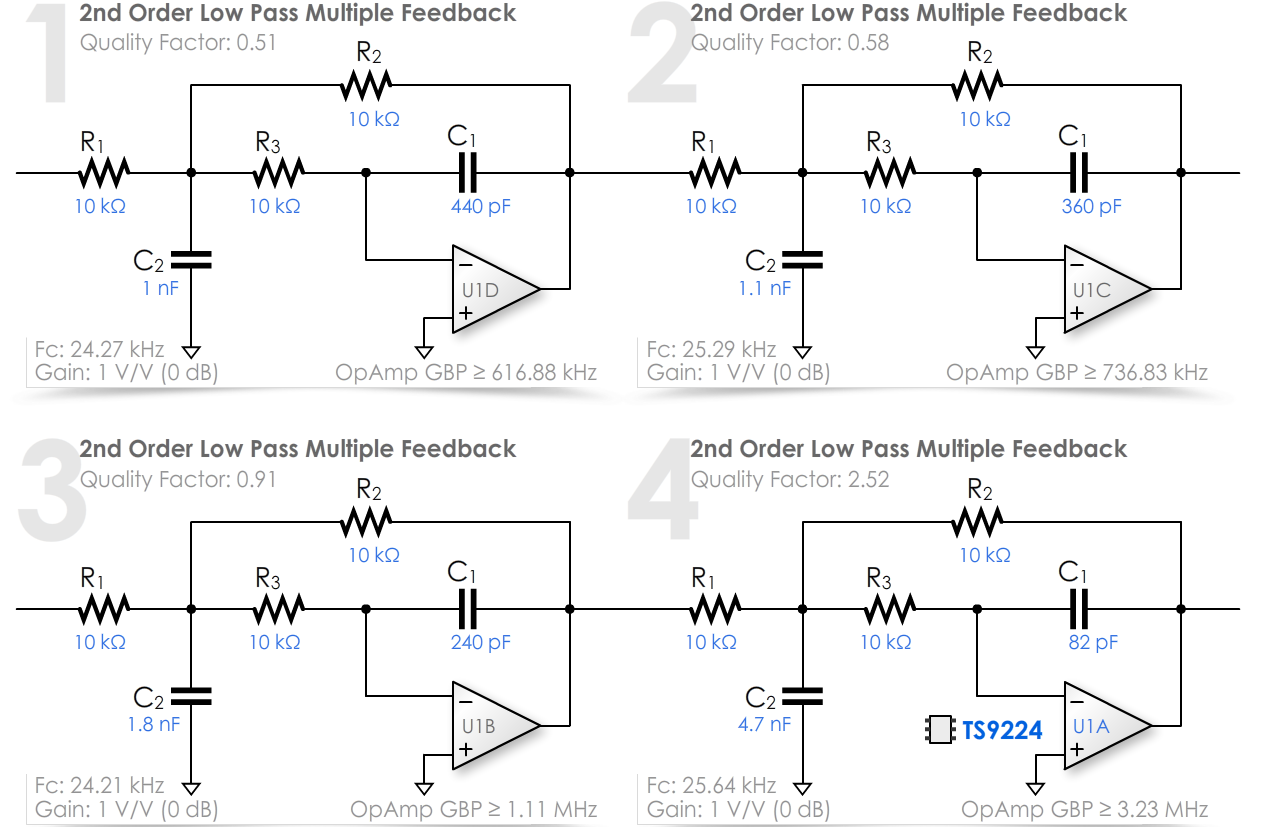
\includegraphics[width=\textwidth]{img/filtro1.png}
\caption{Esquematico}
\end{figure}

\subsection{Componentes activos}

Para elegir el amplificador operacional a utilizar, se usan dos criterios principales\cite{opAmp}\cite{Rules} 

\begin{itemize}
\item El producto Ganancia-Ancho de Banda (GBWP)
\item El Slew Rate
\end{itemize}

En la configuración MFB, el GBWP se calcula como $100(-A_c+1)f_c$ (con $A_c$ la ganancia en lazo cerrado del MFB, en este caso, $A_c=-1$). Por lo tanto, $GBWP \geq 5MHz$.

$SR \geq 2\pi V_{pp}f_c = 2\pi 20V 25kHz = 3.14V/\mu s$

El TL074 cumple con estos requerimientos pues tiene $GBWP=5MHz$ y $SR=13$. Se elige la versión TL074 en el encapsulado SOIC-14 que permite implementar el filtro completo con un solo integrado minimizando el área de la placa impresa. 

\section{Análisis de Ruido a Temperatura Ambiente\cite{Noise}}

Reconocemos tres regiones en el espectro del ruido que afecta a un filtro pasabajos:

\begin{itemize}

\item Ruido rosado o $1/f$
\item Ruido blanco
\item Filtro pasabajos

\end{itemize}

La hoja de datos nos dice que la densidad de ruido de tensión total en $V_{rms}$ es:

$e_n = 4.5nV/\sqrt{Hz}$\\
Y que la densidad de ruido de corriente es de:
$i_n = 0.5pA/\sqrt{Hz}$

Nuestro rango de operación es de $25kHz$, entonces, el ruido a la salida se calcula como 

$e_o = e_n  \sqrt{25kHz}  G = 0.71uV rms$\\
$i_o = i_n \sqrt{kHz} R_{eq} = 1.58uV rms$ (por etapa)
Donde $R_{eq}$ es la resistencia equivalente vista desde la entrada del operacional.

Finalmente calculamos el ruido incorporado por los resistores. Los resistores incorporan ruido térmico, $e_r = \sqrt{ 4 k  T  R_{eq} f_c}$
donde $k$ es la constante de Boltzmann y $T=300K$.

Cada etapa incorpora: 
$\sqrt {4\cdot1.38^{-23} 300K 25kHz 10k\Omega } = 2.04uV rms$

Calculamos el ruido rms para cada etapa:

$(e_n) ^ 2 = (0.71uV)^2 +  (1.58uV) ^2 + (2.04uV)^2 = 7.16 uV^2$

Finalmente calculamos al ruido a la salida 

$N = \sqrt { (e_1)^2 + (e_2)^2 + (e_3)^2 + (e_4)^2 } = 14.32uV rms $

Para tener el ruido $N_{pp}$ a la salida, se lo puede estimar multiplicando el rms por $6$.

$N_{pp} = 85.92uV_{pp}$

Como el rango de entrada es de $20V$ ($\pm 10V$) y la salida de 16 bits, la mitad del bit menos significativo tiene una amplitud de $LSB/2 = 20V/(2*65536) = 152uV$\cite{LSB}. Como $LSB/2 = 152uV$, el ruido no tiene amplitud suficiente para taparlo.

\section{\textbf{Simulación y Medición}}

\subsection{Esquemático del Filtro}

Se presenta el esquemático del prototipo:
 
\begin{figure}[H]
\centering
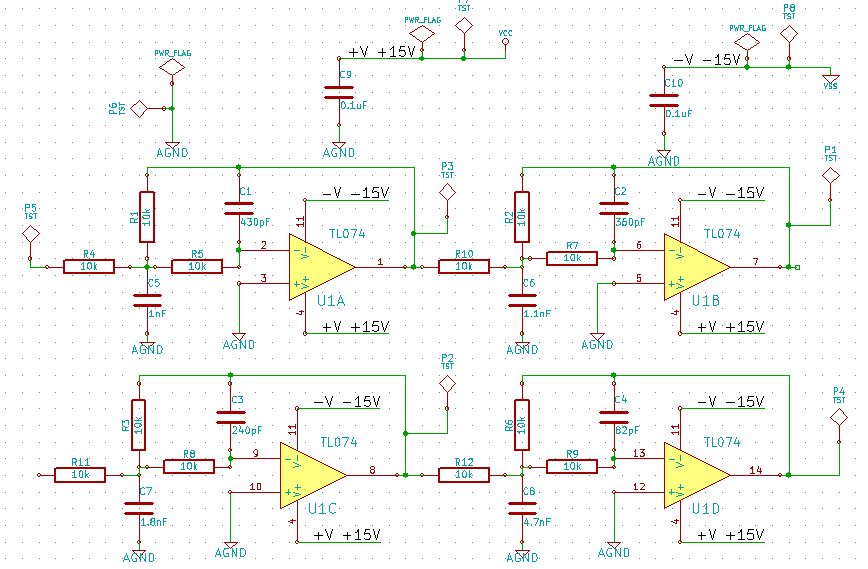
\includegraphics[width=\textwidth]{img/protodrake.png}
\caption{Esquemático del prototipo del filtro}
\end{figure}

Se reproduce el esquemático en el software LTSpice IV, donde se lo somete a simulación.

\begin{figure}[H]
\centering
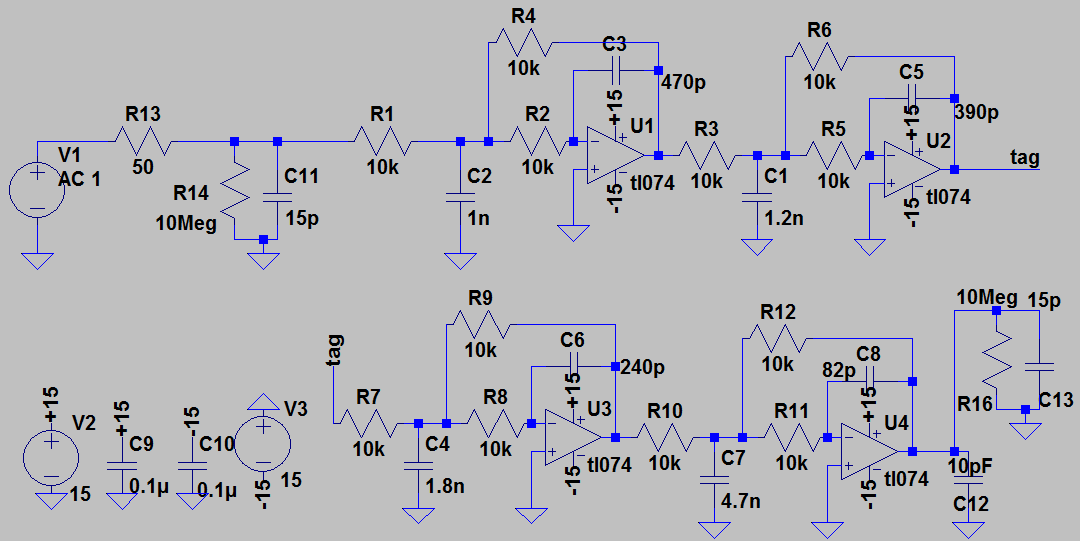
\includegraphics[width=\textwidth]{img/filtro4.png}
\caption{Esquemático de la simulación del filtro}
\end{figure}

El generador de funciones se modela como una fuente $V_1$ en serie con su resistencia interna.
Los efectos de carga del conjunto punta-osciloscopio están modelados como la resistencia $R_{14}$ en paralelo con una capacidad $C_{11}$ a la entrada del filtro.
El efecto de carga de la entrada del conversor a la salida del filtro se obtiene de la siguiente manera:\\
1) La hoja de datos indica una capacitancia de $10pF$ a la entrada del conversor. Esta representada en el esquemático como $C_{12}$\\
2) La hoja de datos no especifica un valor de resistencia sino una alta impedancia de entrada, por lo cual, despreciamos este parámetro en la simulación.

\subsection{Valores de los componentes pasivos}

\begin{tabular}{| l | l | l | l |}
\hline
Resistores & & &\\ \hline
Valor & Tolerancia & Cantidad & Referencia\\ \hline
10$k\Omega$ & 1\% & 8 & $R_{1,\dots ,8}$\\ \hline
Capacitores & & & \\ \hline
Valor & Tolerancia & Cantidad & Referencia \\ \hline
82pF & 5\% & 1 & $C_8$\\ \hline
240pF & 5\% & 1 & $C_6$\\ \hline
390pF & 5\% & 1 & $C_5$ \\ \hline
470pF & 5\% & 1 & $C_3$ \\ \hline
1nF   &	5\% & 1 & $C_2$ \\ \hline
1.2nF & 5\% & 1 & $C_1$ \\ \hline
1.8nF & 5\% & 1 & $C_4$ \\ \hline
4.7nF & 5\% & 1 & $C_7$ \\ \hline
0.1 $\mu F$ & 5\% & 2 & $C_{9,10}$  \\ \hline
\end{tabular}\\

NOTA: Algunos valores de capacidad del diseño por eDesign Suite no se consiguen en el mercado local. Para la implementación se usa el valor comercial más cercano.

\subsection{Banco de Medición}

Banco de Medición:

\begin{figure}[H]
\centering
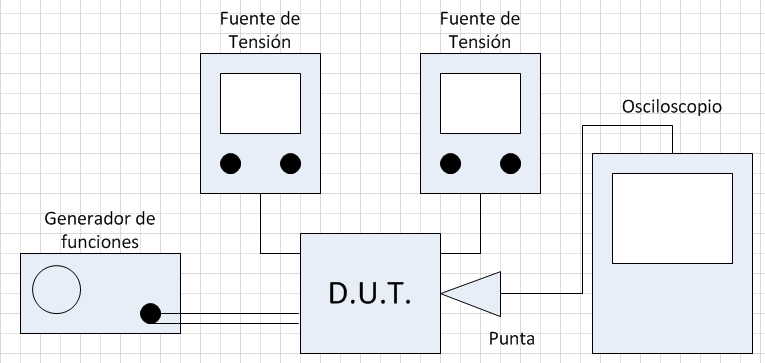
\includegraphics[width=\textwidth]{img/Banco.png}
\caption{Banco de medición}
\end{figure}

\begin{itemize}
\item Fuente de Tensión Fair FR-305A $0-30V$ 
\item Fuente de Tensión Zurich DF1730SB5A $0-30V$
\item Osciloscopio Fluke 192B 60MHz, 500MS/s\\
Sensibilidad 2mV - 100V/div\\
Rango de la base de tiempos: 10 ns - 2 min/div
\item Punta Fluke VP200 10:1 200MHz, 1.000 V CAT II/600 V CAT III (EN61010-1)
\item Generador de Funciones Hing Chang Sweep 9205\\
Frecuencia: $0.02Hz$ a $2MHz$ 7 rangos\\
Precisión: $\pm 5\%$ $(20KHz)$, $\pm 8\% (2MHz)$ 
\end{itemize}

Rise-time del conjunto generador-punta-osciloscopio: $56.8ns$.

\subsection{Imágenes}

<Reservado para foto>

\subsection{Respuesta en frecuencia}

Se realizó un barrido de frecuencias discretas con una señal de entrada senoidal de $10V$ pico, y alimentación de $\pm 15V$. A continuación mostramos los resultados medidos y superpuestos a los valores simulados. Luego de los $50kHz$ el valor de la amplitud era muy bajo para poder seguir realizando mediciones.\\

\begin{tabular}{ l | l | l || l | l | l }
\hline
Frec.(Hz) & Amplitud(V) & Fase(grados) & Frec.(Hz) & Amplitud(V) & Fase(grados) \\   \hline
1 & $10$ & 0 & 4k & $10$& $-47.52$ \\
2 & $10$ & 0 & 5k & $10$& $-61.2$ \\
3 & $10$ & 0 & 6k & $10$& $-75.6$ \\
4 & $10$ & 0 & 7k & $10$& $-88.2$ \\	
5 & $10$ & 0 & 8k & $10$& $-100.8$ \\
6 & $10$ & 0 & 9k & $10$& $-113.4$ \\
7 & $10$ & 0 & 10k & $10.2$& $-126$ \\	
8 & $10$ & 0 & 11k & $10.4$& $-134.64$ \\	
9 & $10$ & 0 & 12k & $10.4$& $-146.88$ \\
10 & $10$ & 0 & 13k & $10.6$& $-163.8$ \\	
20 & $10$ & 0 &14k & $10.6$& $178.56$ \\	
30 & $10$ & 0 &15k & $10.8$& $165.6$ \\
40 & $10$ & 0 &16k & $10.8$& $146.88$ \\	
50 & $10$ & 0 &17k & $11$& $133.56$ \\	
60 & $10$ & 0 &18k & $11$& $113.76$ \\	
70 & $10$ & 0 &19k & $10.8$& $93.24$ \\	
80 & $10$ & 0 &20k & $10.4$& $-72$ \\	
90 & $10$ & 0 &21k & $9.8$& $-52.92$ \\	
100 & $10$ & 0 &22k & $8.8$& $31.32$ \\	
200 & $10$ & 0 &23k & $7.6$& $12.24$ \\	
300 & $10$& 0 &24k & $6.4$& $-25.92$ \\	
400 & $10$& $-7.2$ &25k & $5.2$& $-31.5$ \\	
500 & $10$& $-7.2$ &26k & $4$& $-56.16$ \\	
600 & $10$& $-0.864$ &27k & $3.6$& $-54.43$ \\			
700 & $10$& $-1$ &28k & $2.4$& $-88.7$ \\	
800 & $10$& $-1.15$ &29k & $2$& $-79.34$ \\	
900 & $10$& $-12.96$ &30k & $1.6$& $-95.04$ \\
1k & $10$& $-11.52$ &40k & $0.2$& $-167.04$ \\	
2k & $10$& $-24.48$ &50k & $0.04$& $-169.2$ \\
3k & $10$& $-38.88$ &
\end{tabular}

\begin{figure}[H]
\centering
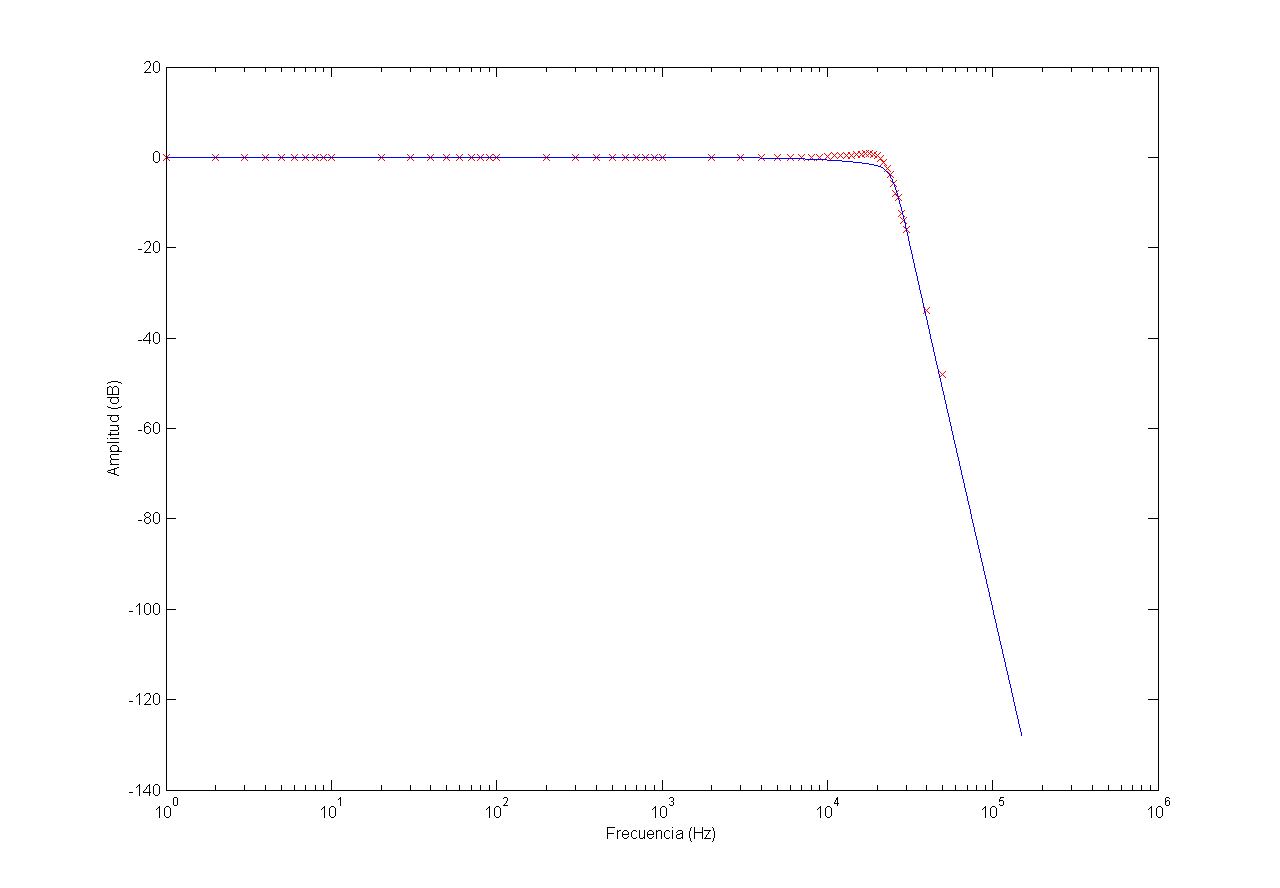
\includegraphics[width=\textwidth]{img/amp.png}
\caption{Respuesta en amplitud. Simulación (azul) y medición (rojo)}
\end{figure}
\begin{figure}[H]
\centering
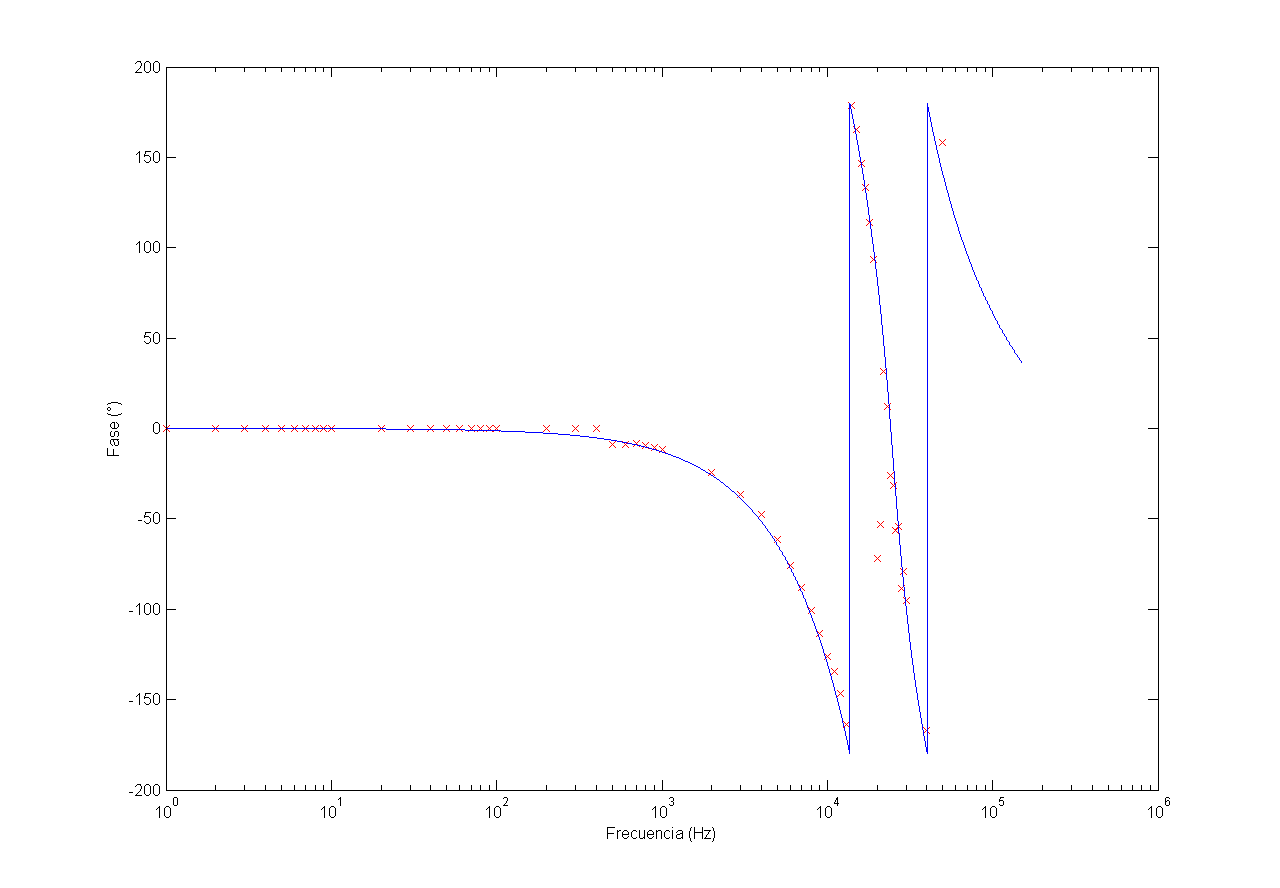
\includegraphics[width=\textwidth]{img/fase.png}
\caption{Respuesta en fase. Simulación (azul) y medición (rojo)}
\end{figure}

\subsection{Respuesta al escalón}

Se fija como entrada un pulso largo de $-10V$ a $10V$ y se mide el rise-time (tiempo transcurrido entre el $10\%$ y el $90\%$ de la transición de estado bajo a estado alto de la señal) a la salida del filtro. En la simulación se definió el rise-time de la fuente como el valor de rise-time medido del conjunto generador-punta-osciloscopio. Se muestran los resultados comparando con la simulación.

\begin{figure}[H]
\centering
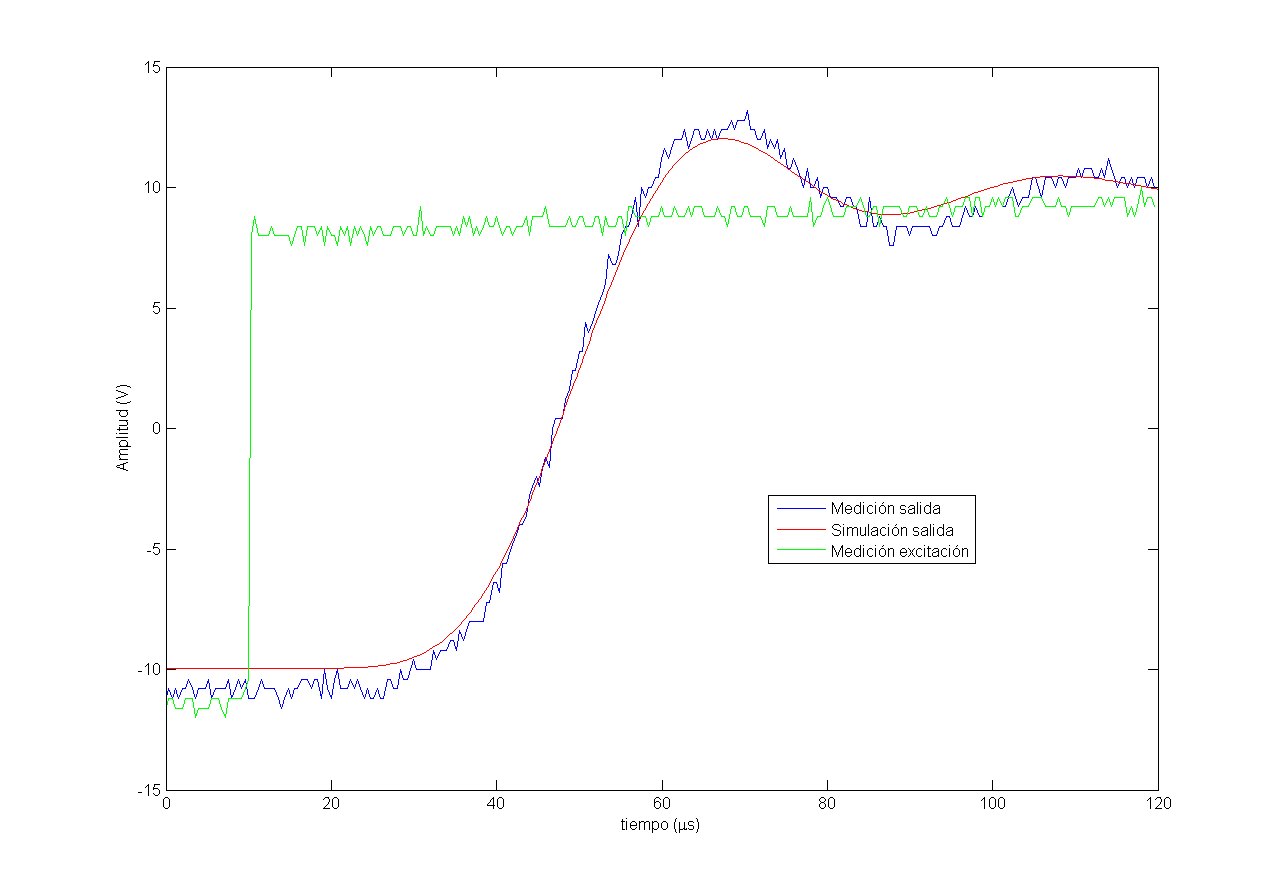
\includegraphics[width=\textwidth]{img/escalon.png}
\caption{Respuesta al escalon. Simulación (rojo) y medición (azul)}
\end{figure}

Rise-time de la simulación: $20.64\mu s$.\\
Rise-time de la medición: $20\mu s$.\\

\subsection{Imágenes}

<Reservado para foto>

\newpage
\begin{thebibliography}{99}

\bibitem{RM}Ron Mancini - Texas Instruments, \textit{Op Amps for Everyone. Application Report SLOD006B}, Agosto 2002.

\bibitem{LSB}Martin Mason - Electronic Design, \textit{The ABCs Of ADCs}, Septiembre 2009.

\bibitem{SNR}\textit{MT-001: Taking the Mystery out of the Infamous Formula, "SNR=6.02N + 1.76dB," and Why You Should Care}, 2009, Walt Kester - Analog Devices.

\bibitem{BB}Bonnie Baker - Microchip Technology, \textit{Anti-Aliasing, Analog Filters for Data Acquisition Systems, AN699}, 1999.

\bibitem{MFB}Jim Karki - Texas Instruments, \textit{Active Low-Pass Filter Design. Application Report SLOA049B}, Septiembre 2002. 

\bibitem{eDS}\url{http://www.st.com/edesignsuite}. Ultima visita: 18/03/14.

\bibitem{opAmp}Bonnie C. Baker - Microchip Technology, \textit{Select the Right Operational Amplifier for your Filtering Circuits}, 2003.

\bibitem{Rules}G. Hall, \textit{"Rules" of low noise amplifier}, Noviembre 2001.

\bibitem{Noise}Art Kay - Texas Instruments, \textit{Op-Amp Noise Calculation and Measurement}, 2005.

\end{thebibliography}

\end{document}


